\chapter{Análisis del problema y solución propuesta}

\section{Restricciones, alternativas y decisión}
Una comparación útil debe distinguir tres niveles: interpolaciones simples, un conjunto pequeño de
modelos preentrenados con papeles científicos diferentes y, únicamente si la validación lo
justifica, una adaptación acotada. Se descarta recopilar muchos modelos sin profundidad analítica y
también se descarta convertir una aplicación, el tratamiento de PDF o el reconocimiento óptico de
música en requisito del núcleo experimental.

La solución aplicada fue una comparación controlada y reproducible sobre entradas emparejadas,
seguida de una adaptación secundaria de EDSR. La comparación principal permaneció intacta; para la
adaptación se asignaron otros grupos de fuente SMB a roles de entrenamiento, validación y prueba
sin solapamiento de páginas ni identificadores. Esta separación operativa no garantiza independencia
entre composiciones completas, pues distintos grupos pueden corresponder a movimientos de una
misma obra. Una vez asegurados ambos estudios se admitió una extensión acotada: un demostrador
local y una prueba sin reajuste sobre obras externas. Cada comparación compartió condiciones y
reglas de agregación dentro de su propio denominador, y la interpretación integró fidelidad,
errores de notación, recursos, licencias y restricciones operativas.
La Tabla~\ref{tab:alternatives} resume las opciones consideradas y la razón por la que cada una se
incorporó, aplazó o excluyó.

\begin{table}[htbp]
  \centering
  \footnotesize
  \setlength{\tabcolsep}{3pt}
  \caption{Alternativas valoradas antes de cerrar el alcance. Fuente: elaboración propia.}
  \label{tab:alternatives}
  \begin{tabular}{p{0.20\textwidth}p{0.23\textwidth}p{0.24\textwidth}p{0.23\textwidth}}
    \toprule
    Alternativa & Valor que aportaba & Coste o amenaza & Decisión \\
    \midrule
    Bicúbica únicamente & Referencia rápida y explicable & No representa un método aprendido & Incluir como línea base, no como única solución \\
    EDSR y SwinIR preentrenados & Dos familias y pesos oficiales para x2/x4 & Transferencia desde imágenes naturales & Incluir y auditar fallos musicales \\
    Modelos perceptuales o difusión & Mayor realismo aparente & Alucinación, más coste y menor trazabilidad & Excluir del núcleo orientado a fidelidad \\
    Ajuste fino & Posible adaptación al dominio & Riesgo de fuga y coste adicional & Ejecutar un estudio secundario acotado tras asegurar el núcleo \\
    Demostrador y piloto externo & Evidencia tangible de aplicabilidad & Nueva pregunta, derechos y revisión adicional & Ejecutar una extensión acotada después de asegurar el núcleo \\
    PDF, OMR o despliegue & Flujo de producto o tarea posterior & Validación y riesgos distintos & Mantener como trabajo futuro \\
    \bottomrule
  \end{tabular}
\end{table}

\section{Riesgos técnicos y científicos}
El primer riesgo era la contaminación del benchmark: inspeccionar resultados, ajustar umbrales o
seleccionar modelos con la muestra principal de SMB habría invalidado su papel de evaluación final.
El control adoptado mantuvo
el conjunto bloqueado hasta congelar manifiesto, métodos, puntos de control, degradaciones,
métricas, exclusiones, muestreo y reglas de interpretación.

Otros riesgos fueron la desalineación entre entrada y referencia, la pérdida de denominadores por
errores de procesado y la falsa precisión al tratar páginas o regiones de una misma obra como
observaciones independientes. Se conservaron los fallos explícitos, se verificó el emparejamiento
y se agrupó por identificador de fuente SMB. Este control no elimina la posible dependencia entre
movimientos o ediciones relacionados, que limita la interpretación de los intervalos.

Los métodos perceptuales y generativos pueden producir detalle visualmente plausible sin garantizar
su correspondencia con la fuente \cite{ledig2017srgan,wang2018esrgan,kim2026fidesr}.
% Claim evidence: SOTA-PERCEPTION-DISTORTION, SOTA-CURRENT-GENERATIVE-RISK
Por ello, una mejora agregada no bastó: se revisaron pentagramas, símbolos, dígitos y texto, y se
retuvieron también ejemplos negativos. Los riesgos de tiempo, memoria y energía se registraron por
ejecución y justificaron detener extensiones opcionales antes de comprometer el núcleo o el margen
de entrega.
La matriz de la Tabla~\ref{tab:risk-matrix} conecta estos riesgos con sus controles y con el
resultado realmente observado, incluido el fallo del primer protocolo de degradación.

\begin{table}[htbp]
  \centering
  \footnotesize
  \setlength{\tabcolsep}{3pt}
  \caption{Riesgos principales, controles aplicados y resultado. Fuente: elaboración propia a
  partir del registro de riesgos del proyecto.}
  \label{tab:risk-matrix}
  \begin{tabular}{p{0.22\textwidth}p{0.10\textwidth}p{0.10\textwidth}p{0.29\textwidth}p{0.19\textwidth}}
    \toprule
    Riesgo & Prob. & Impacto & Control & Resultado \\
    \midrule
    Contaminar la prueba & Media & Crítico & Congelación previa y separación por ID de fuente; 64 grupos principales excluidos de la adaptación & Sin IDs compartidos; dependencia entre movimientos no descartada \\
    Degradación no transferible & Media & Crítico & Calibración visual y trazas por página & Ocurrió en v1; corregido y repetido como v2 \\
    Métricas favorables con error musical & Media & Crítico & Revisión cualitativa fija y regla de contradicción & Ocurrió en casos; limita la recomendación \\
    Peso, licencia o entorno incompatible & Media & Alto & Fuentes oficiales, hashes y prueba Kaggle & Resuelto antes de la ejecución final \\
    Coste o plazo excesivo & Alta & Crítico & Núcleo primero y extensión acotada a EDSR & Controlado; se preservó la evaluación \\
    Derechos por imagen insuficientes & Media & Alto & Separar acceso, procesamiento y reproducción; documentar base, atribución y proporcionalidad & Comparaciones seleccionadas; la autorización del archivo no acredita todos los derechos \\
    \bottomrule
  \end{tabular}
\end{table}

\section{Marco legal, ético y medioambiental}
La documentación oficial de SMB informa de acceso controlado y licencia CC BY-NC 4.0
\cite{martinez2025smb,smbDatasetCard,ccByNc40}, pero esa etiqueta no se interpretó automáticamente
como autorización ilimitada para redistribuir cualquier escaneo o transformación. Deben separarse
la licencia del conjunto, la procedencia y derechos de cada partitura, las licencias del código y
los pesos, y la base que permite publicar cada figura. La memoria utiliza SMB con atribución,
finalidad académica no comercial e indicación de las transformaciones; reproduce recortes y una
única comparación de página completa elegida de antemano porque resulta necesaria para explicar el
comportamiento global del sistema. El resto del conjunto y los paneles completos no se
redistribuyen. La reproducción se integra en el análisis y juicio crítico, identifica la obra y la
fuente y se limita a la extensión justificada por ese propósito. El artículo 32.1 de la
Ley de Propiedad Intelectual \cite{boeLpiArticle32} se considera como base de cita y análisis,
sujeta a sus requisitos en cada reproducción. No se presupone que la licencia del conjunto
resuelva por sí sola todos los derechos de cada edición o digitalización.

En el piloto externo, la Societat Joventut Musical d'Albal (SJMA) autorizó el acceso, procesamiento
y reproducción en el TFG de las doce páginas de prueba aportadas. La memoria muestra el conjunto
cualitativo externo completo ---ocho casos aceptados, tres con reservas y un rechazo--- como
fragmentos instrumentales de obras de banda, vinculados directamente a comparaciones y comentarios
críticos. Se atribuyen obra, autor
o arreglista, parte e institución de procedencia; no se publican las otras cuatro páginas recibidas,
el corpus bruto ni las restantes salidas. La autorización institucional y este uso analítico
acotado no se describen como cesión ni
como titularidad del estudiante sobre las obras, arreglos o ediciones. La custodia del archivo y
su autorización no acreditan por sí solas todos los derechos de reproducción pública de terceros;
la base aplicable debe valorarse para cada imagen, especialmente en las páginas completas.

La evaluación consideró como amenazas las representaciones insuficientes de fuentes, estilos de grabado,
densidades de notación, tamaños de pentagrama, tipografías y calidades de digitalización. También se
evitaron afirmaciones de beneficio universal o de reconocimiento no medido. El principal riesgo
ético es presentar una reconstrucción inventada como documento fiel, con posibles consecuencias
para consulta, interpretación, edición o conservación. El análisis medioambiental registró
hardware, duración y consumo computacional pertinente en lugar de asumir que un modelo más complejo
es profesionalmente preferible.

No se trataron datos personales ni se entrenó un sistema de decisión sobre personas, por lo que no
se identificó un tratamiento de categorías personales ni un riesgo de discriminación individual.
Sí existe un sesgo documental: solo se estudió notación impresa compatible con SMB y la selección
final exigió una escala de pentagrama mensurable. El piloto añadió partes de banda de otra
colección, pero no manuscritos, tradiciones de notación no representadas, entradas LR naturales
heterogéneas ni páginas que el estimador no pudo caracterizar. La consecuencia ética no es asignar
un resultado a una persona, sino ofrecer peor cobertura o una falsa
sensación de fidelidad para determinados documentos.

\section{Plan de trabajo y recursos}
El trabajo se organiza en incrementos de evidencia: contrato y gobierno de SMB; degradaciones e
interpolaciones; selección y validación de modelos; evaluación controlada; y síntesis, reproducción
y depósito. El núcleo científico tuvo prioridad; solo después de reconciliarlo se añadieron la
adaptación acotada de EDSR y, como última extensión separable, el piloto externo con demostrador
local. El tratamiento de PDF, OMR, despliegue, nuevas familias y mejoras no esenciales permanecen
fuera del alcance. La contingencia final se reserva para comentarios de los
revisores, correcciones invalidantes, reproducción limpia y operaciones de depósito.

La planificación inicial asignó 330 horas al TFG. Al no existir un parte horario contemporáneo,
se realizó una reconstrucción retrospectiva por paquetes de trabajo, contrastada con los hitos,
artefactos, ejecuciones y revisiones conservados. La estimación de referencia, anterior al piloto
externo y a las tareas finales de cierre, es
de 346 horas, con un intervalo prudente de 312 a 380 horas. La distribución central fue de 64 horas
para el contrato, el estado del arte y el gobierno de SMB; 73 para el diseño experimental y las
líneas base; 71 para integrar los modelos y ejecutar la adaptación acotada; 82 para las dos ejecuciones SMB,
la corrección del protocolo y el análisis; y 56 para la memoria y su control de calidad. Se estiman
22 horas adicionales para incorporar las dos revisiones, cerrar el depósito y preparar la defensa,
lo que situó la previsión previa en 368 horas. El piloto profesional recibió después una envolvente
adicional de 10--16 horas, de modo que la previsión final pasa a 378--384 horas sin atribuir como
dedicación del estudiante el tiempo de cómputo no supervisado. Estas cifras
expresan dedicación académica estimada, no una medición cronográfica, y por ello se comunica también
su incertidumbre.
La Figura~\ref{fig:effort} contrasta la distribución por fases con el plan inicial; sus barras
cubren esa estimación de referencia, mientras que la previsión final de
378--384 horas incorpora también el cierre y el piloto profesional.

Frente al plan, la evaluación consumió más por detectar que la primera degradación no se transfería
a páginas completas, normalizarla por la escala del pentagrama y repetir el experimento. La
adaptación secundaria añadió unas 20 horas una vez protegido el núcleo. Antes del piloto, la
previsión aumentaba 38 horas (un 11,5\,\%) respecto de las 330 iniciales y rebasaba en 8 horas el
límite superior del intervalo orientativo de 300--360 horas asociado a los 12 ECTS; la extensión
eleva la diferencia prevista a 48--54 horas. Se comunica la desviación en lugar de ajustar
retrospectivamente el esfuerzo al intervalo. Los recursos materiales fueron el equipo local ya
disponible, Overleaf y una GPU gratuita de Kaggle; no se imputa un coste salarial ficticio ni un
gasto no documentado.

\begin{figure}[htbp]
  \centering
  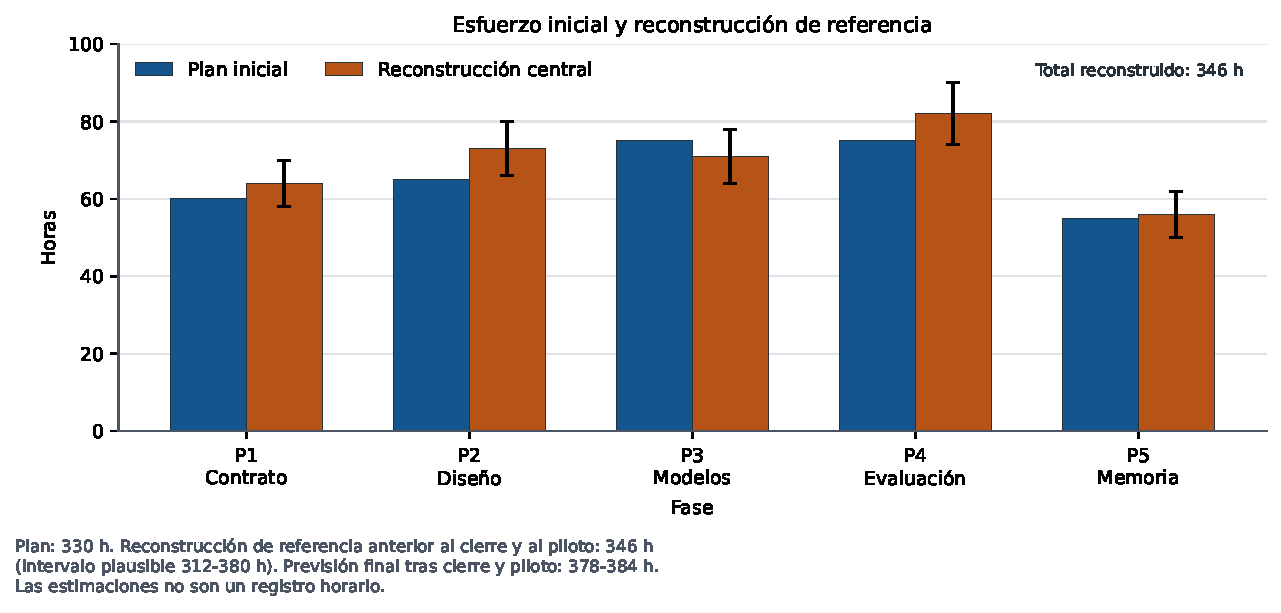
\includegraphics[width=\textwidth]{figures/context/effort-plan-vs-reconstruction.pdf}
  \caption{Comparación entre el plan inicial y la reconstrucción retrospectiva por fase. Las barras
  de error expresan el intervalo plausible, no variabilidad estadística; la figura cubre 346 horas
  centrales de referencia, no las 378--384 horas previstas tras el cierre y el piloto.
  Fuente: elaboración propia a partir del registro de esfuerzo.}
  \label{fig:effort}
\end{figure}

\begin{table}[htbp]
  \centering
  \small
  \caption{Recursos y costes directos planificados. Fuente: elaboración propia.}
  \label{tab:resources-cost}
  \begin{tabular}{p{0.27\textwidth}p{0.37\textwidth}p{0.22\textwidth}}
    \toprule
    Recurso & Uso & Coste incremental \\
    \midrule
    Equipo local disponible & Desarrollo, auditoría, pruebas y análisis & 0 € de adquisición; 20--80 € estimados de electricidad y red \\
    Kaggle con Tesla T4 & Inferencia aprendida acotada & 0 € en el plan ejecutado \\
    Overleaf y TeX Live local & Edición autoritativa y prevalidación & 0 € incremental \\
    Almacenamiento y copias & Datos restringidos y artefactos fuera de Git & 0--30 € de contingencia \\
    Impresión y trámites & Solo si el proceso vigente lo exige & 0--50 € provisionales \\
    \midrule
    Total externo & Rango de planificación; no gasto acreditado & 20--160 € \\
    \bottomrule
  \end{tabular}
\end{table}

La Tabla~\ref{tab:resources-cost} separa la dedicación académica de los costes directos externos.
El trabajo del estudiante se expresa en horas y no se monetiza con una tarifa inventada. Del mismo
modo, disponer de una cuota gratuita no equivale a coste ambiental nulo: al no medirse energía, el
análisis se limita a duración, hardware y decisiones de reducción de cálculo.
